KisTA enables the export of a TiKZ file, which in turn, can be compiled into an image
to show the activity of the tasks and of the schedulers.
%
This report has several advantages compared to the VCD report.
\begin{enumerate}
\item The user can configure the bounds of the analysis, that is, when the trace starts and how many
time stamps along the time line will be shown where consequtive events occur 
\footnote{
The VCD trace is done over the whole simulation, which can be heavy and not very practical for long simulation runs}.
The philosophy is to report the activity which fits in a piece of paper.
\item The report reflects the events in their order of appearance without implying a proportional separation of events.
This is useful to represent sequence of events where some intervals are much larger than others.
\item The report can be edited (under the widely supported TiKZ format) by the user, e.g. to change styles, colors, remove or add details, etc,
 before compiling the final image.
\item The report can be easily used for documentation, since it can be easily inserted in a LaTeX document or converted to an image format.
\end{enumerate}

%
The export of the TiKZ activity report can be enabled and configured from both
the C/C++ API and the KisTA XML front-end.
%
KisTA provides methods and options for enabling and configuring the activity report
from both front-ends, which reduces the need for editing the resulting TiKZ file.

\subsubsection{Using the C++ API}
\label{sec:activity_c_api}

Listing~\ref{list:2tasks_tikz_trace} shows a first example of how to enable and control the export of an activity report.
It is an excerpt from the example \texttt{tikz\_tracing\_and\_sched\_times\_ex1} available with the KisTA library.
All the functions and code shown have to be called before the simulation start (call to \texttt{sc\_start}).
\begin{table}[htbp]
\begin{lstlisting}[style=KistaCodeStyle,caption={API for controling tracing tasks and scheduler activity.},label=list:2tasks_tikz_trace]
   ...
   tikz_activity_trace_handler gen_tikz_report_handler;

   gen_tikz_report_handler = create_tikz_activity_trace("2tasks_tikz_trace");
   
   set_scale(gen_tikz_report_handler,1);
   set_landscape(gen_tikz_report_handler);
   do_not_show_unactive_boxes(gen_tikz_report_handler);
   set_time_stamps_max_separation(gen_tikz_report_handler,3);

   ...

\end{lstlisting}
\end{table}

The user has to declare a handler of type \texttt{tikz\_activity\_trace\_handler} for each activity trace one wants to generate.
Several traces (e.g. starting at different times and/or comprising a different number of events) can be configured.
%
To effectively generate the trace, the \texttt{create\_tikz\_activity\_trace} function has to be called.
The function returns a handler of type \texttt{tikz\_activity\_trace\_handler}, which is used later on by the
configuration functions to specify the activity report they refer to.
%
The \texttt{create\_tikz\_activity\_trace} function admits also a string as a parameter to specify a name for the activity report file.
For instance, in the Listing~\ref{list:2tasks_tikz_trace} example, a file named \texttt{2tasks\_tikz\_trace.tex} file will be generated.
If no string parameter is provided, a unique name, based on the prefix \texttt{tikz\_activity\_trace} is assigned.

In this example, the use of some additional configuration functions are illustrated.
For instance, the \texttt{set\_scale} method enables to control de size of the exported sketch.
In this case, the command is redundant, because the default scale is 1.00.

The function \texttt{set\_landscape} enables a \emph{landscape} format of the report.
The default format is \emph{portrait}.

After executing the simulation and runing the \texttt{pdflatex} command on the \texttt{2tasks\_tikz\_trace.tex} file,
the resulting pdf document is shown in Figure~\ref{fig:2tasks_tikz_trace}.
\begin{figure}[htbp]
\centering
%\includegraphics[width=\textwidth]{./figs/.png} 
\fbox{
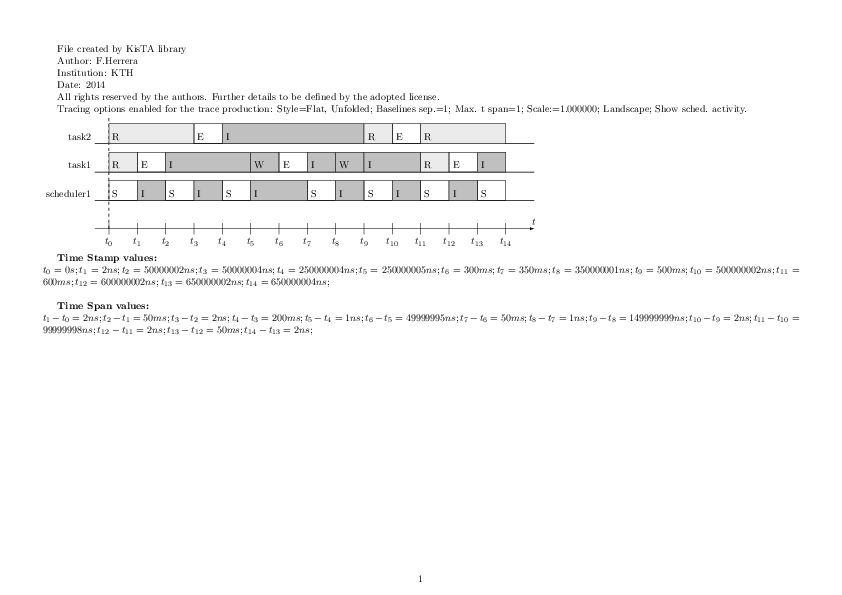
\includegraphics[width=0.75\textwidth]{./figs/2tasks_tikz_trace.png} 
}
\caption{Two tasks tikz activity trace from the \texttt{tikz\_tracing\_and\_sched\_times\_ex1} example with the configuration of Listing~\ref{list:2tasks_tikz_trace}.} 
\label{fig:2tasks_tikz_trace}
\end{figure}

The trace has two text parts plus the activity diagram.
A first text header reports the generation source and the configuration (including the default values) of the activity trace.
%
Then, below, the activity diagram is shown.
In this example, the two tasks and the scheduler are represented in the trace.
As can be seen, the trace includes by default 15 events.
Any state change in any of the tasks or in the scheduler is considered as an event.
As can be observed too, by default, the trace equally spaces the events, no mater the time elapsed between consecutive events.

By default, two consecutive state changes are delimited by a box.
The box has a colour code depending on the state.
For tasks, a running state is coloured in white; a ready-to-execute state in a light grey, while the
remaining states (blocking on communication, waiting for time, etc) in a dark grey.
For schedulers, a scheduling state (the scheduler is computing) is coloured in white,
while an inactive state is coloured in dark-grey.

Finally, the report also dumps the absolute times associated to each event, 
and the time spans of consecutive events.

\begin{figure}[htbp]
\centering
%\includegraphics[width=\textwidth]{./figs/.png} 
\fbox{
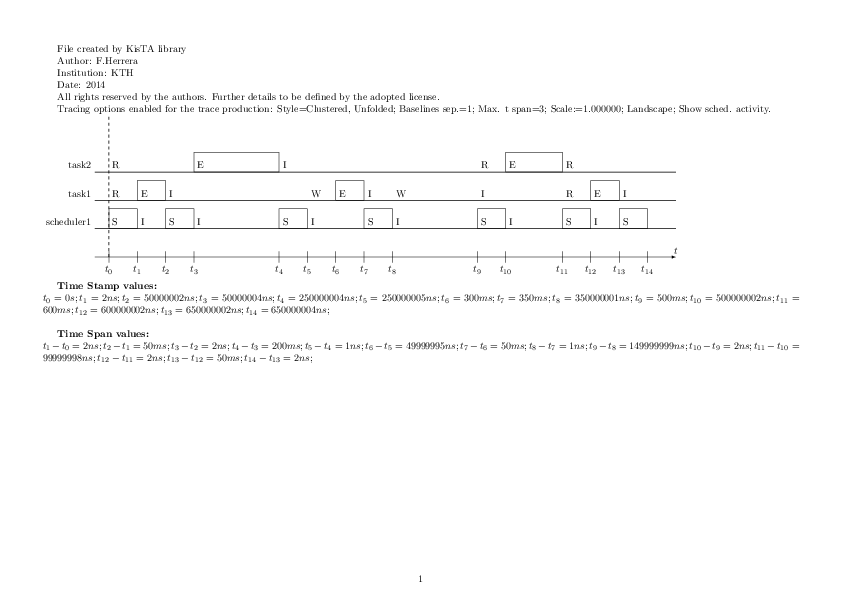
\includegraphics[width=0.75\textwidth]{./figs/2tasks_tikz_trace_2.png} 
}
\caption{Two tasks tikz activity trace from the \texttt{tikz\_tracing\_and\_sched\_times\_ex1} example with the configuration of Listing~\ref{list:2tasks_tikz_trace}.} 
\label{fig:2tasks_tikz_trace_2}
\end{figure}

Figure~\ref{fig:2tasks_tikz_trace_2} shows a variant where the activity report with the configuration of Listing~\ref{list:2tasks_tikz_trace}.
Such a configuration has added the calls to \texttt{do\_not\_show\_unactive\_boxes} and to \texttt{set\_time\_stamps\_max\_separation}.

The function \texttt{do\_not\_show\_unactive\_boxes} states that all the boxes representating states where the tasks is not computing
are not represented.
Therefore, only white boxes corresponding to the intervals where the task is computing are represented.
%
For schedulers, the call to \texttt{do\_not\_show\_unactive\_boxes} means that only the 
white boxes corresponding to the intervals where the scheduler task is computing, that is in scheduling state, are represented.

The function \texttt{set\_time\_stamps\_max\_separation} enables a non-homogeneous separation among
consecutive events in the diagram, but with a limit in the maximum number of separation units in the diagram.
This way the diagram roughly shows the differences in the time spans, while still focused on the sequence of events 
(regardless the actual times) and makes feasible to show a number of events.
For instance, in the Listing~\ref{list:2tasks_tikz_trace}, the second parameter is 3, which means that the activity diagram
can use up to 3 spaces in the diagram for longer intervals.
In Figure~\ref{fig:2tasks_tikz_trace_2}, three spaces are used for the $(t_3t_4)$ interval, which takes $200ms$,
while the $(t_2t_3)$ interval, which takes $2ns$, and which makes the actual time span ratio is of several orders of magnitud.
%
Using a proportional scale would have meant that either $t_4$ events would go beyond the limits of the diagram,
or that $(t_2t_3)$ interval would be undistinguisable from a point in time.

There are also options to facilitate the export of the diagram (without informative text) and its reuse in a document.
For instance,  Listing~\ref{list:2tasks_tikz_only_img} shows a configuration to export only the image.
For it, the \texttt{only\_image} function is used.
Additionally,  Listing~\ref{list:2tasks_tikz_only_img} also shows the use of the \texttt{no\_text\_in\_traces},
which removes from the diagram the codes showing the new state of the task (or scheduler) after the event.
%
Finally, in Listing~\ref{list:2tasks_tikz_only_img} example, the scale has been changed to extend
the picture to the width limits of the A4 portrait format.
%

\begin{table}[htbp]
\begin{lstlisting}[style=KistaCodeStyle,caption={API for controling tracing tasks and scheduler activity.},label=list:2tasks_tikz_only_img]
   ...
   tikz_activity_trace_handler gen_tikz_report_handler;
   gen_tikz_report_handler = create_tikz_activity_trace("2tasks_tikz_trace");
   
   set_scale(gen_tikz_report_handler,1.25);
   set_landscape(gen_tikz_report_handler);
   no_text_in_traces(gen_tikz_report_handler);
   do_not_show_unactive_boxes(gen_tikz_report_handler);
   set_time_stamps_max_separation(gen_tikz_report_handler,3);
   only_image(gen_tikz_report_handler);
   ...
\end{lstlisting}
\end{table}

The result of the configuration of Listing~\ref{list:2tasks_tikz_only_img} is shown in Figure~\ref{fig:2tasks_tikz_only_img}.
The black borders do not appear in the report.
In Figure~\ref{fig:2tasks_tikz_only_img} they illustrate the limit of the A4 portrait format.
 
\begin{figure}[htbp]
\centering
%\includegraphics[width=\textwidth]{./figs/.png} 
\fbox{
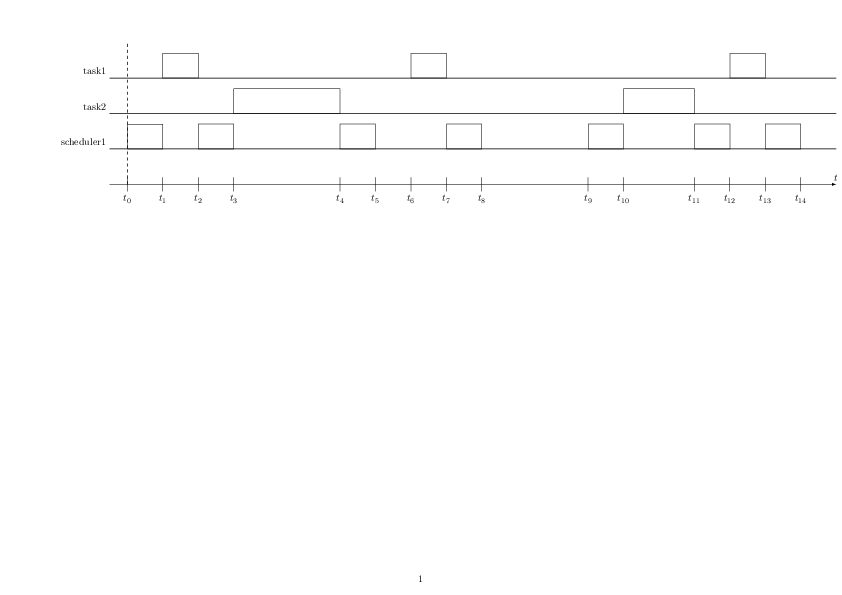
\includegraphics[width=0.75\textwidth]{./figs/2tasks_tikz_only_img.png} 
}
\caption{Two tasks tikz activity trace from the \texttt{tikz\_tracing\_and\_sched\_times\_ex1} example with the configuration of Listing~\ref{list:2tasks_tikz_only_img}.} 
\label{fig:2tasks_tikz_only_img}
\end{figure}

In order to get a tighter fit, the produced .tex file can be edited, through the configuration of the \texttt{figure} LaTeX environment.
%
Another possibility is to edit the figure in pdf format (after running \texttt{pdflatex})
or in .png or .jpeg format, through a simple cut,
to obtain something as shown in Figure~\ref{fig:2tasks_tikz_only_img_ed}.

\begin{figure}[htbp]
\centering
%\includegraphics[width=\textwidth]{./figs/.png} 
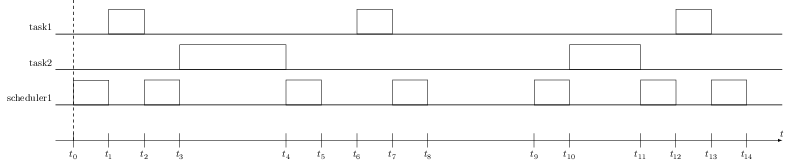
\includegraphics[width=0.75\textwidth]{./figs/2tasks_tikz_only_img_ed.png} 
\caption{Two tasks tikz activity trace from the \texttt{tikz\_tracing\_and\_sched\_times\_ex1} example with the configuration of Listing~\ref{list:2tasks_tikz_only_img} and edited.} 
\label{fig:2tasks_tikz_only_img_ed}
\end{figure}

The previous examples show only a part of the configuration possibilities of the activity report facilitated
by KisTA.

Following, the available configuration functions are described in a systematic way.

Functions for control of the trace sampling:
\begin{itemize}
\item \texttt{void set\_start\_time(tikz\_activity\_trace\_handler handler, sc\_time start\_time)}:\\
can be used to set the time where the trace starts to be sampled.
If this function is not called, the default start time, stated by the variable \texttt{DEFAULT\_TIKZ\_TRACE\_START\_TIME\_NS} (tipically 0) is taken.
\item \texttt{void set\_max\_number\_of\_time\_stamps(tikz\_activity\_trace\_handler handler, \\
 unsigned int max\_time\_stamps);}:
\\ can be used to set the end of the trace sampling through a user-defined maximum number of time stamps where a new event occur.
If this function is not called, the default number of time stamps, stated by the variable \texttt{DEFAULT\_TIKZ\_TRACE\_EVENTS\_LIMIT} (typically 15) is taken.
\end{itemize}

Functions for format configuration:
\begin{itemize}
\item \texttt{void set\_scale(tikz\_activity\_trace\_handler handler, float scale)}:\\
Function to set the scale of the figure. The default value is stated by the
variable \texttt{DEFAULT\_TIKZ\_TRACE\_SCALE} (tipically 1.00).
    
\item \texttt{ void set\_landscape(tikz\_activity\_trace\_handler handler)}:\\
Function to export the diagram in a landscape format.
The default format (if this function is not called) is a \emph{portrait} format.
\end{itemize}

Functions for format configuration:
\begin{itemize}
\item \texttt{void do\_not\_show\_schedulers(tikz\_activity\_trace\_handler handler)}:\\
If this function is called, the activity corresponding to the schedulers is not shown.
By default, the schedulers activity is also shown (in the default \emph{unfolded style}).

\item \texttt{void no\_text\_in\_traces(tikz\_activity\_trace\_handler handler)}:\\
If this function is called, informative labels within the activity boxes are not shown.
These informative labels are shown by default.
They show the state of the task or of the scheduler in the unfolded style.

\item \texttt{void do\_not\_show\_unactive\_boxes(tikz\_activity\_trace\_handler handler)}:\\
If this function is called, the activity diagram shows boxes only for the execution states
in the task activities, and for the scheduling state in the scheduler activities.
By default (if this function is not called), activity boxes are shown for every 
state.
Then, execution and scheduling state boxes are filled in white.
For the unfolded format, different grays are used for the remaining states.
For tasks, light greys are used for ready-to-execute states, while 
dark grey for blocking states.

\item \texttt{void only\_image(tikz\_activity\_trace\_handler handler)}:\\
If this function is used, only the diagram showing tasks and scheduler activities.
By default, if this function is not called, a textual information is added.
This information is composed of a header, which includes the configuration of the
exported activity diagram, 
and a tail information with the time stamps and the time intervals.

\item \texttt{void set\_base\_lines\_separation(tikz\_activity\_trace\_handler handler, unsigned int separation)}:\\
This function serves to control de separation of the base lines used to represent task and scheduler activities.
The default base lines separation is stated by the variable \texttt{DEFAULT\_TIKZ\_TRACE\_BASE\_LINES\_SEPARATION},
and it is typically 1.

\item \texttt{void set\_time\_stamps\_max\_separation(tikz\_activity\_trace\_handler handler,\\
 unsigned int max\_separation)}:\\
This function can be used for enabling a non-homogeneous separation among consecutive time stamps,
and at the same time, to define the maximum separation, so the intervals do not need to be proportionally represented.
The default max. separation is stated by the variable \texttt{DEFAULT\_TIKZ\_TIME\_STAMPS\_MAX\_SEPARATION},
and it is typically 1.
\end{itemize}

\subsubsection{Activity diagrams for a multiprocessor system models with the C++ API}
\label{sec:activity_multiproc_c_api}

Additionally, there are other two functions which are useful for organizing and compacting the 
the activity diagrams, specially in an multi-processor environment:

\begin{itemize}
\item \texttt{void cluster(tikz\_activity\_trace\_handler handler)}:\\
When this function is called, the activity diagram cluster the traces
based on the task-to-scheduler mapping.
Each cluster groups one scheduler together with all the tasks which have
been mapped to the scheduler.
If neither, this function, nor the \texttt{compact} function, are called,
the \texttt{unfolded format} is applied by default.
Under the unfolded format, all the tasks activities are shown first,
and the scheduler activities (if their representation is not disabled
with \texttt{do\_not\_show\_schedulers} function.

\item \texttt{void compact(tikz\_activity\_trace\_handler handler)}:\\
The call to this function makes effect when the \texttt{cluster} function is called.
When the compact function is called, the \texttt{compact style} for the 
clustered representation is used.
A compact clustered representation of an activity diagram uses
one trace (one base line) for representing the utilization of each scheduler.
The trace represents either the execution of the scheduler, or the execution
of some of the tasks assigned to the scheduler, or a blocking or inactivity
state where neither the scheduler, nor any of its assigned tasks are executing.
\end{itemize}

Section~\ref{sec:activity_xml} shows examples of clustered and compact diagrams.

\subsubsection{Using the XML front-end}
\label{sec:activity_xml}

All the options for enabling and configuring activity reports are also available
from the KisTA XML front-end.
Example of Listing~\ref{list:activity_report_1} shows a first configuration example
for the Voice Activity Detection (VAD) example distributed within the KisTA library.

\begin{table}[htbp]
\begin{lstlisting}[language=XML, caption={Example of configuration of an activity report from the XML interface for the VAD example.}, label=list:activity_report_1]
<kista_configuration>
  <analysis>
    ...
    <!-- TiKZ trace  -->
    <!-- "file" states the name of the tikz trace file, plus .tex -->
    <tikz_trace enabled="true" name="tikz_trace">
	<!-- all the next configuration parameters of the tikz trace -->
        <!-- are optional and have default values -->
	<!-- control of trace sampling and time axis separation-->
	<start_time value="9" unit="ms" />
	<max_number_of_time_stamps value="16"/>
	<time_stamps_max_separation value="3"/>

	<!-- control of vertical axis information -->
	<cluster value="true" compact="false"/>
	<base_lines_separation value="1"/>

	<!-- control of information in the draw -->
	<no_text_in_traces value="true"/>
	<do_not_show_unactive_boxes value="true"/>	
	<!-- -->
	<do_not_show_schedulers value="false"/>	
			
	<!-- control of picture format -->
	<set_scale value="0.75"/>
	<set_landscape value="true"/>
			
        <only_image value="true"/>
    </tikz_trace>
    ...
  </analysis>
</kista_configuration>
\end{lstlisting}
\end{table}

Running \texttt{ kista-xml} application with the Listing~\ref{list:activity_report_1} configuration produces
a .tex file, which in turns, after applying pdflatex, produces the diagram shown in Figure~\ref{fig:tikz_trace_only_img1}.


\begin{figure}[htbp]
\centering
%\includegraphics[width=\textwidth]{./figs/.png} 
\fbox{
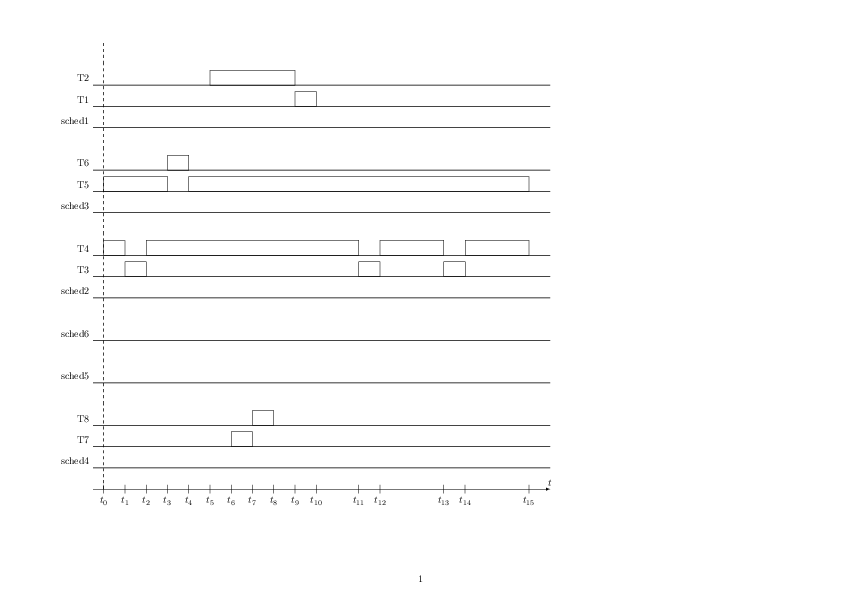
\includegraphics[width=\textwidth]{./figs/tikz_trace_only_img1.png} 
}
\caption{Tikz activity trace of the VAD example with the XML configuration of Listing~\ref{list:activity_report_1}.} 
\label{fig:tikz_trace_only_img1}
\end{figure}

In Listing~\ref{list:activity_report_2} some slight changes on the configuration of Listing~\ref{list:activity_report_1},
which are summarized as:
\begin{itemize}
\item print, as well as the diagram image, the header text with configuration options, and tail text, showing task names alias used for the diagram, time stamp values,
and time interval values (disabling \texttt{only\_image} option),
\item print boxes for all states with grey backgrounds to mark unactive and blocking states (disabling \texttt{<do\_not\_show\_unactive\_boxes value="true"/>}),
\item enable the compact (as well as clustered) format (\texttt{compact="true"}),
\item print text labels corresponding to the active task or scheduler running (for compact state) (disabling \texttt{<no\_text\_in\_traces value="true"/>}).
\end{itemize}
 
\begin{table}[htbp]
\begin{lstlisting}[language=XML, caption={Example of configuration of an activity report from the XML interface for the VAD example.}, label=list:activity_report_2]
<kista_configuration>
  <analysis>
    ...
    <!-- TiKZ trace  -->
    <!-- "file" states the name of the tikz trace file, plus .tex -->
    <tikz_trace enabled="true" name="tikz_trace">
	<!-- all the next configuration parameters of the tikz trace -->
        <!-- are optional and have default values -->
	<!-- control of trace sampling and time axis separation-->
	<start_time value="9" unit="ms" />
	<max_number_of_time_stamps value="16"/>
	<time_stamps_max_separation value="3"/>

	<!-- control of vertical axis information -->
	<cluster value="true" compact="true"/>
	<base_lines_separation value="1"/>

	<!-- -->
	<do_not_show_schedulers value="false"/>	
			
	<!-- control of picture format -->
	<set_scale value="0.75"/>
	<set_landscape value="true"/>
    </tikz_trace>
    ...
  </analysis>
</kista_configuration>
\end{lstlisting}
\end{table}

The resulting activity report exported by KisTA is shown in Figure~\ref{fig:tikz_trace_only_img2}.

\begin{figure}[htbp]
\centering
\fbox{
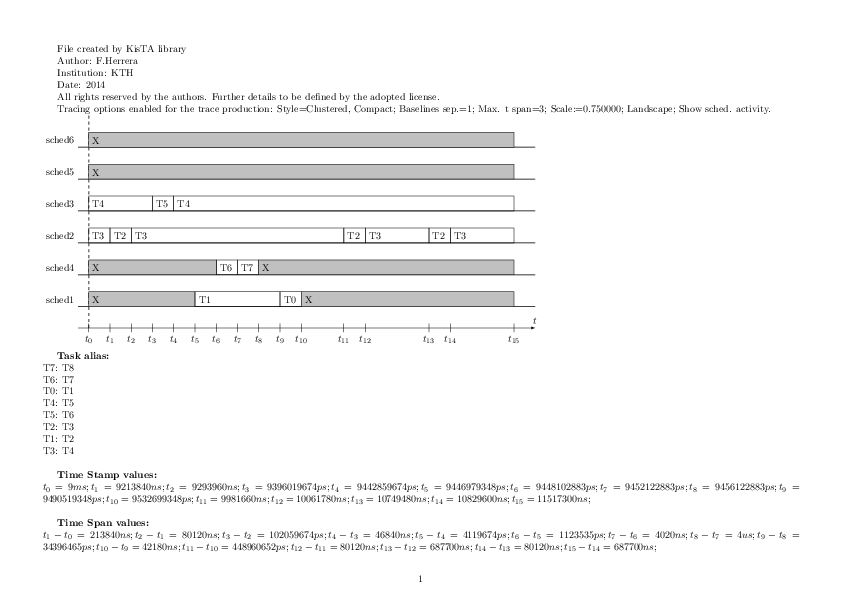
\includegraphics[width=\textwidth]{./figs/tikz_trace_only_img2.png} 
}
\caption{Tikz activity trace of the VAD example with the XML configuration of Listing~\ref{list:activity_report_2}.} 
\label{fig:tikz_trace_only_img2}
\end{figure}


